% \documentclass{article}
% \usepackage{graphicx} % Required for inserting images

% \title{COL774 A3 Writeup}
% \author{Aman Hassan}
% \date{November 2023}

% \begin{document}

% \maketitle

% \section{Introduction}

% \end{document}

\documentclass[12pt]{article}
\usepackage[a4paper,margin=0.75in]{geometry}
\usepackage[utf8]{inputenc}
\usepackage[OT1]{fontenc}
\usepackage[table,usenames,dvipsnames]{xcolor}
\usepackage{array}
\usepackage{varwidth}
\usepackage{tabularx}
\usepackage{amsmath}
\usepackage{hyperref}
\usepackage{enumitem}
\usepackage{graphicx}
\usepackage{tcolorbox}
\renewcommand*\familydefault{\sfdefault}

\newtcolorbox{mybox}[3][]
{
  colframe = #2!25,
  colback  = #2!10,
  coltitle = #2!20!black,  
  title    = {#3},
  #1,
}

\hypersetup{
    colorlinks=true,
    linkcolor=blue,
    filecolor=magenta,      
    urlcolor=cyan,
    pdftitle={Overleaf Example},
    pdfpagemode=FullScreen,
}

\title{\textbf{COL774 Assignment 3}}
\author{Aman Hassan \\ \texttt{2021CS50607}}
\date{November 2023}

\begin{document}

\maketitle

\section{Decision Tree}

\begin{enumerate}[label=(\alph*)]
  
    \item Here we constructed the Decision Tree for varying depths where features to split are determined using highest mutual information metric
    \begin{enumerate}[label=\roman*.]
        \item 
            \begin{itemize}
                \item Only Win:
                \begin{itemize}
                    \item Accuracy for in prediction type of only win on training set is 50.3380
                    \item Accuracy for in prediction type of only win on test set is 49.6380
                \end{itemize}
                \item Only Loss
                \begin{itemize}
                    \item Accuracy for in prediction type of only loss on training set is 49.6614
                    \item Accuracy for in prediction type of only loss on test set is 50.3619
                \end{itemize}
                \item DT with varying depths on training set:
                \begin{itemize}
                    \item Accuracy for depth 5 on training set is 88.5652
                    \item Accuracy for depth 10 on training set is 99.7828
                    \item Accuracy for depth 15 on training set is 99.8466
                    \item Accuracy for depth 20 on training set is 99.8466
                    \item Accuracy for depth 25 on training set is 99.8466
                    \item Accuracy for depth 30 on training set is 99.8466
                \end{itemize}
                \item DT with varying depths on test set:
                \begin{itemize}
                    \item Accuracy for depth 5 on test set is 57.6008
                    \item Accuracy for depth 10 on test set is 60.1861
                    \item Accuracy for depth 15 on test set is 60.1861
                    \item Accuracy for depth 20 on test set is 60.1861
                    \item Accuracy for depth 25 on test set is 60.1861
                    \item Accuracy for depth 30 on test set is 60.1861
                \end{itemize}
            \end{itemize}
        From the data obtained we find that single type prediction(only win, only loss) performs worse compared to Decision Tree classification (DT is almost 2x better in training prediction). As we expect the training accuracy is much better than test accuracy. We also find that the accuracy is almost the same after depth 10-15 ( This can be attributed to the aggressive terminating conditions applied on grow\_tree / fit function ) 
        \item The following Accuracy vs depth graph was obtained
    \end{enumerate}
    \begin{center}
        \begin{tabular}{c}
            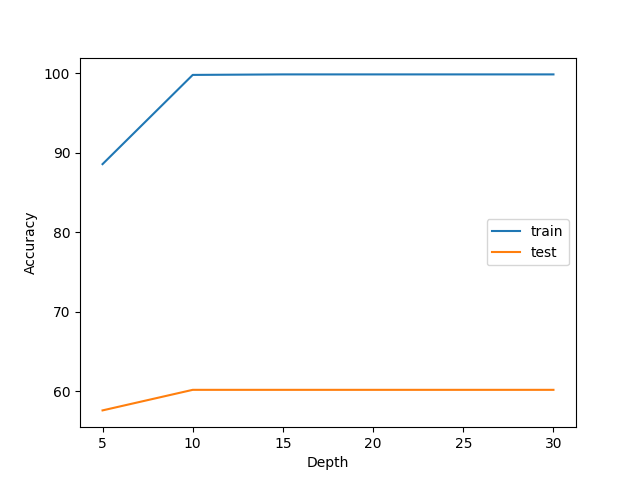
\includegraphics[width=0.9\textwidth]{Graphs/Q1/a.png}
        \end{tabular}
    \end{center}
    
    \item Using one-hot encoding we obtain the following results

    \begin{enumerate}[label=\roman*.]
        \item 
            \begin{itemize}
                \item Only Win:
                \begin{itemize}
                    \item Accuracy for in prediction type of only win on training set is 50.3386
                    \item Accuracy for in prediction type of only win on test set is 49.6381
                \end{itemize}
                \item Only Loss
                \begin{itemize}
                    \item Accuracy for in prediction type of only loss on training set is 49.6614
                    \item Accuracy for in prediction type of only loss on test set is 50.3619
                \end{itemize}
                \item DT with varying depths on training set:
                \begin{itemize}
                    \item Accuracy for depth 15 on training set is 70.6018
                    \item Accuracy for depth 25 on training set is 84.9112
                    \item Accuracy for depth 35 on training set is 92.5514
                    \item Accuracy for depth 45 on training set is 99.1057
                \end{itemize}
                \item DT with varying depths on test set:
                \begin{itemize}
                    \item Accuracy for depth 15 on test set is 55.9462
                    \item Accuracy for depth 25 on test set is 61.7373
                    \item Accuracy for depth 35 on test set is 61.5305
                    \item Accuracy for depth 45 on test set is 61.5305
                \end{itemize}
            \end{itemize}
        From the data obtained we find that Decision Tree classification performs better compared to single type prediction(only win, only loss). As we expect the training accuracy is much better than test accuracy for a given depth. However contrary to part (a) we find that here the accuracies significantly increase as we increase the depth for the case of training set and for the test set, it increases from 15 to 25, decreases from 25 to 35 and then remains same for the next increment of depth. 
        \item The following Accuracy vs depth graph was obtained
    \end{enumerate}
    \begin{center}
        \begin{tabular}{c}
            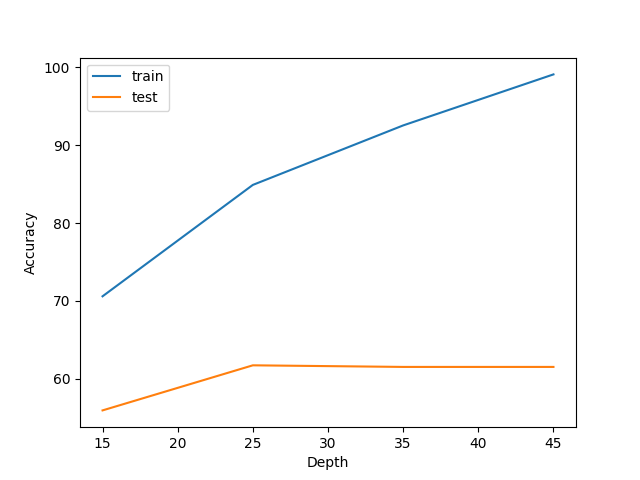
\includegraphics[width=0.9\textwidth]{Graphs/Q1/b.png}
        \end{tabular}
    \end{center}
        


    
    \item The following Accuracy vs nodes graphs were obtained upon performing reduced error pruning for various depths

    \begin{center}
        \begin{center}
        \begin{tabular}{c c}
            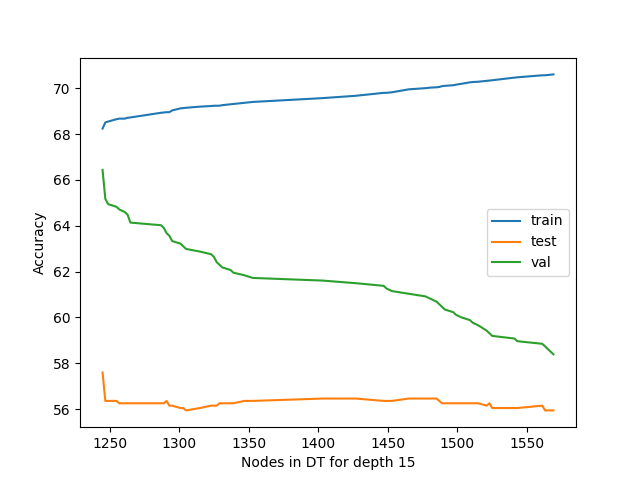
\includegraphics[width=0.45\textwidth]{Graphs/Q1/c_15.png} & 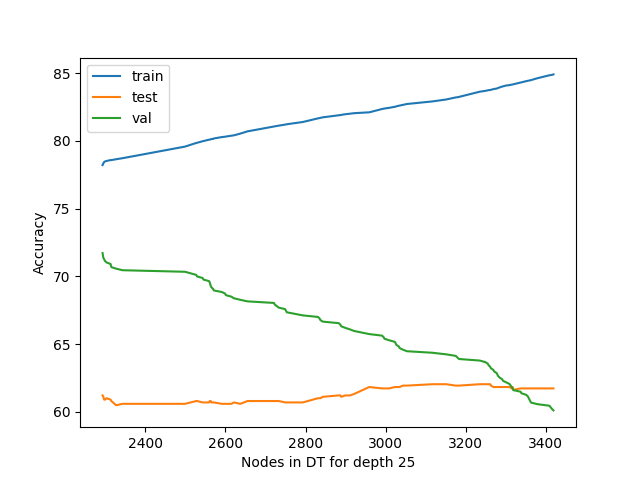
\includegraphics[width=0.45\textwidth]{Graphs/Q1/c_25.png} 
        \end{tabular}
        \begin{tabular}{c c}
            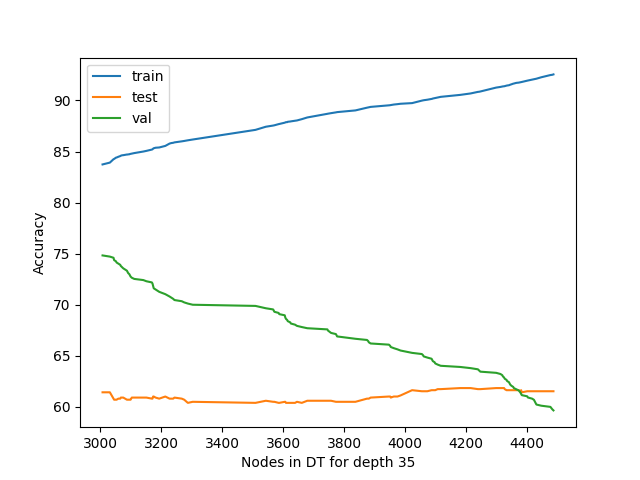
\includegraphics[width=0.45\textwidth]{Graphs/Q1/c_35.png} & 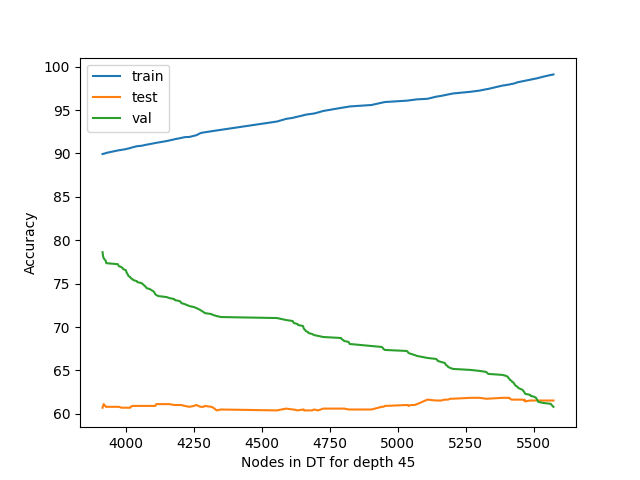
\includegraphics[width=0.45\textwidth]{Graphs/Q1/c_45.png} 
        \end{tabular}
        \end{center}
    \end{center}

    Some observations to note:
    \begin{itemize}
        \item In all graphs the training accuracy decreases as number of nodes reduce in the graph (which suggests that more nodes could possibly lead to overfitting)
        \item Both the validation increases as number of nodes reduce in the graph 
        \item we find that the test accuracies remain around the same value throughout the process
        \item In the initial stage of the DT (before pruning) we find the following order of accuracies:
        \begin{itemize}
            \item For depth 15: train \textgreater val \textgreater test accuracy
            \item For all other depths: train \textgreater test \textgreater val accuracy
        \end{itemize}
        \item As more nodes are pruned we find the following order of accuracies: train \textgreater val \textgreater test
    \end{itemize}
    

\item Decision Tree using sci-kit learn

\begin{enumerate}[label=\roman*.]
    \item Varying Max-Depth
    \begin{itemize}
        \item Training Set Accuracies:
        \begin{itemize}
            \item Training Accuracy for max\_depth = 15 is 71.3428
            \item Training Accuracy for max\_depth = 25 is 85.4734
            \item Training Accuracy for max\_depth = 35 is 94.3529
            \item Training Accuracy for max\_depth = 45 is 99.5528
        \end{itemize}
        \item Test Set Accuracies:
        \begin{itemize}
            \item Test Accuracy for max\_depth = 15 is 60.5998
            \item Test Accuracy for max\_depth = 25 is 63.3919
            \item Test Accuracy for max\_depth = 35 is 64.6329
            \item Test Accuracy for max\_depth = 45 is 64.0124
        \end{itemize}
    \end{itemize}
    \newpage
     The obtained graph is as follows:
     \begin{center}
        \begin{tabular}{c}
            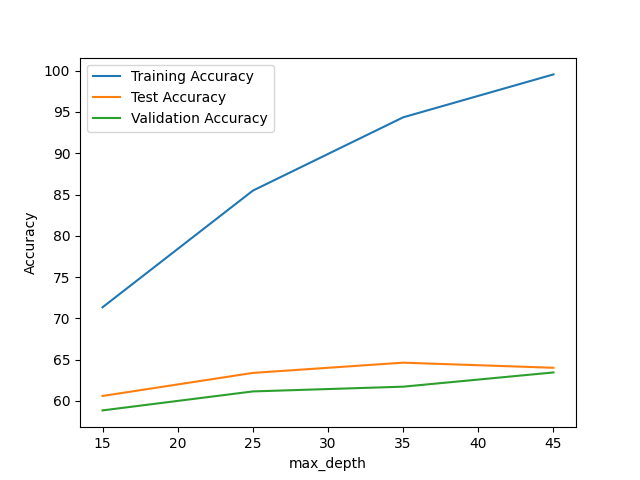
\includegraphics[width=0.9\textwidth]{Graphs/Q1/d_max_depth.png}
        \end{tabular}
    \end{center}
    We find that the best max\_depth obtained using the validation set is 45
    \item Varying ccp\_alpha
    \begin{itemize}
        \item Training Set Accuracies:
        \begin{itemize}
            \item Training Accuracy for ccp\_alpha = 0.001 is 68.9408
            \item Training Accuracy for ccp\_alpha = 0.01 is 53.4432
            \item Training Accuracy for ccp\_alpha = 0.1 is 50.3386
            \item Training Accuracy for ccp\_alpha = 0.2 is 50.3386
        \end{itemize}
        \item Test Set Accuracies:
        \begin{itemize}
            \item Test Accuracy for ccp\_alpha = 0.001 is 66.2875
            \item Test Accuracy for ccp\_alpha = 0.01 is 51.8097
            \item Test Accuracy for ccp\_alpha = 0.1 is 49.6381
            \item Test Accuracy for ccp\_alpha = 0.2 is 49.6381
        \end{itemize}
    \end{itemize}
    \newpage
    The obtained graph is as follows:
    \begin{center}
        \begin{tabular}{c}
            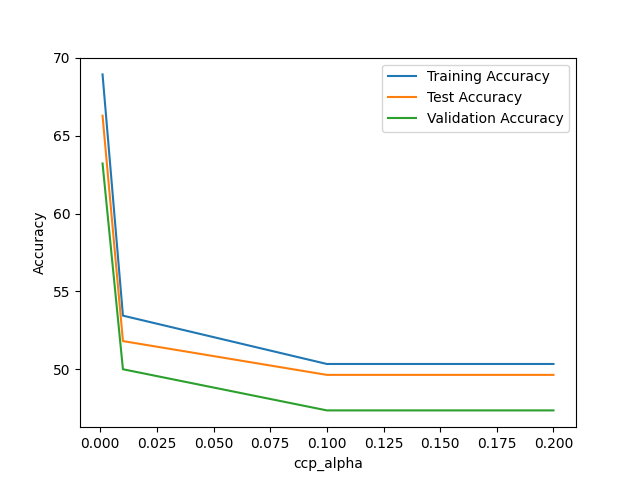
\includegraphics[width=0.9\textwidth]{Graphs/Q1/d_ccp_alpha.png}
        \end{tabular}
    \end{center}
     We find that the best ccp\_alpha obtained using the validation set is 0.001
    \item Observations to note:
    \begin{itemize}
        \item We find that the training data prediction accuracy is lesser in the sci-kit learn model compared to the model developed in both part b and c
        \item On the other hand we find that the test data prediction accuracy is hifher in the sci-kit model as compared to the model developed in both b and c
    \end{itemize}
\end{enumerate}

\item Random Forests



\end{enumerate}

\clearpage

\section{Neural Networks}

\begin{enumerate}[label=(\alph*)]
    \item \begin{enumerate}[label=\roman*.]
        \item With a threshold of $\alpha_i > 10^{-6}$ for the support vectors. We obtain the following results for a linear kernel
        \begin{itemize}
            \item No of support vectors: 673
            \item \% of support vectors wrt training examples: 14.138655462184873\%
        \end{itemize}
        \item The test accuracy we obtain is 94.0\%
        \item The top 6 support vectors are:

        \begin{center}
        \begin{tabular}{c c c}
            
\includegraphics[width=0.2\textwidth]{Images/Q2_binary/linear_sv_1.png} &
            
\includegraphics[width=0.2\textwidth]{Images/Q2_binary/linear_sv_2.png} &
            
\includegraphics[width=0.2\textwidth]{Images/Q2_binary/linear_sv_3.png} \\
        \end{tabular}
        \begin{tabular}{c c c}
            
\includegraphics[width=0.2\textwidth]{Images/Q2_binary/linear_sv_4.png} &
            
\includegraphics[width=0.2\textwidth]{Images/Q2_binary/linear_sv_5.png} &
            
\includegraphics[width=0.2\textwidth]{Images/Q2_binary/linear_sv_6.png} \\
        \end{tabular}
        \end{center}

        The weight image obtained is:

        \begin{center}
            
\includegraphics[width=0.2\textwidth]{Images/Q2_binary/linear_w.png} 
        \end{center}
    \end{enumerate}

    \item \begin{enumerate}[label=\roman*.]
        \item With a threshold of $\alpha_i > 10^{-6}$ for the support vectors. We obtain the following results for a Gaussian Kernel
        \begin{itemize}
            \item No of support vectors: 1067
            \item \% of support vectors wrt training examples: 22.415966386554622\%
            \item Number of support vectors that match in both linear and gaussian: 571
        \end{itemize}
        \item The test accuracy we obtain is 94.25\%
        \item The top 6 support vectors are:

        \begin{center}
        \begin{tabular}{c c c}
            
\includegraphics[width=0.2\textwidth]{Images/Q2_binary/gaussian_sv_1.png} &
            
\includegraphics[width=0.2\textwidth]{Images/Q2_binary/gaussian_sv_2.png} &
            
\includegraphics[width=0.2\textwidth]{Images/Q2_binary/gaussian_sv_3.png} \\
        \end{tabular}
        \begin{tabular}{c c c}
            
\includegraphics[width=0.2\textwidth]{Images/Q2_binary/gaussian_sv_4.png} &
            
\includegraphics[width=0.2\textwidth]{Images/Q2_binary/gaussian_sv_5.png} &
            
\includegraphics[width=0.2\textwidth]{Images/Q2_binary/gaussian_sv_6.png} \\
        \end{tabular}
        \end{center}
    \item We see that the validation accuracy obtained in Gaussian kernel is slightly higher than that of linear kernel (0.25\% higher)
    \end{enumerate}

    \item \begin{enumerate}[label=\roman*.]
        \item Number of Support Vectors obtained is as follows
        \begin{itemize}
            \item Linear Kernel: sklearn\_svm has 669 SV's over CVXOPT's 673 SV's
            \item Gaussian Kernel: sklearn\_svm has 1056 SV's over CVXOPT's 1067 SV's
        \end{itemize}
        \begin{center}
            \begin{tabular}{c c}
                & CVXOPT \\
                Scikit & 
            \begin{tabular}{c|c|c|}
                    & lin  & rbf  \\   
                \hline
                lin & 669 & 569 \\
                \hline
                rbf & 566 & 1056 \\
                \hline
            \end{tabular}
            \end{tabular}
        \end{center}

    \item Comparison of weight and bias in linear kernel:
    \begin{itemize}
        \item CVXOPT: b = -4.0888424817486575
        \item sklearn\_svm: b = -4.0881856782113015
        \item norm(w\_cv - w\_skl) = 0.015257845622513772
    \end{itemize}
    \item Validation set accuracy is as follows:
    \begin{itemize}
        \item Linear Kernel: sklearn\_svm obtains 94.75\% accuracy over CVXOPT's 94\% accuracy
        \item Gaussian Kernel: sklearn\_svm obtains 93.75\% accuracy over CVXOPT's 94.25\% accuracy
    \end{itemize}

        \item The training times are given below:
            \begin{center}
                \begin{tabular}{|l|c|}
                    \hline
                    Scikit RBF & 1.649s (+ 23.210s for data retrieval) \\
                    Scikit linear & 1.944s (+ 22.590s for data retrieval)\\
                    CVXOPT RBF & 154.257s (+ 23.080s for data retrieval)\\
                    CVXOPT linear & 81.493s (+ 24.363s for data retrieval)\\
                    \hline
                \end{tabular}
            \end{center}
    \end{enumerate}

\end{enumerate}

\section{Multiclass SVM}

\begin{enumerate}[label=(\alph*)]
    \item Using the previously created CVXOPT Solver we obtain 55.414\% accuracy in Multi-class classification
    \item Using the scikit SVM library we obtain 56.083\% accuracy on the same test set. We also see that in comparison to CVXOPT, the scikit SVM library is much faster. The exact time taken to train the model is as follows 2028.495s (\~ 33 mins) for CVXOPT implementation in comparison to 53.316s (\~ 1 min) for scikit library. Note the accuracy rate is almost similar (differing only by \~0.53\%)

    \item The confusion matrices for both implementations is as follows:
    \begin{center}
        \begin{tabular}{c c}
            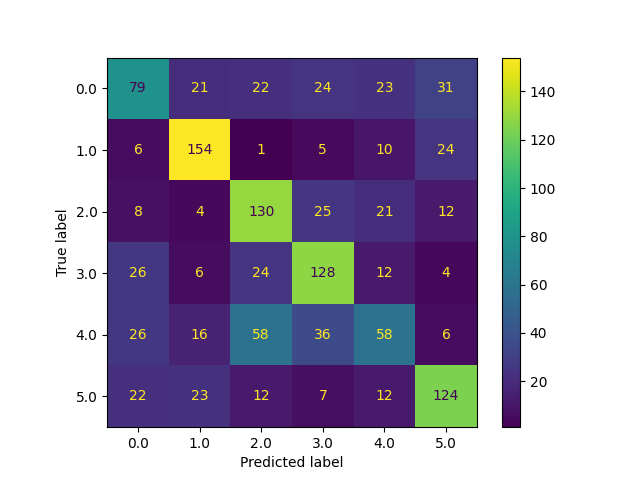
\includegraphics[width=0.44\textwidth]{Images/Q2_multi/confusion_sklearn.png} & 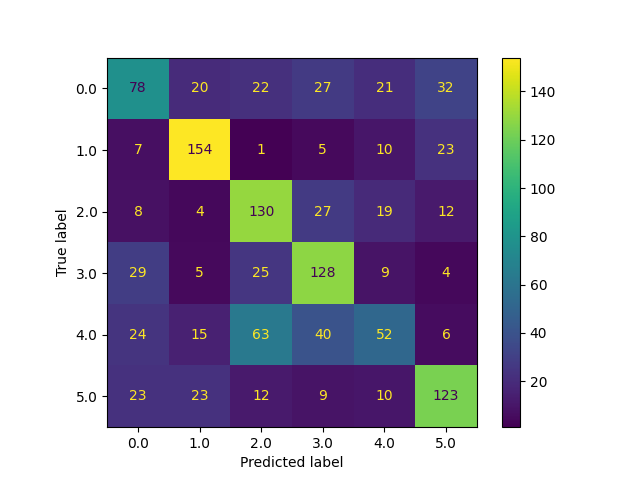
\includegraphics[width=0.44\textwidth]{Images/Q2_multi/confusion_cvxopt.png} \\
            Scikit & CVXOPT 
        \end{tabular}
    \end{center}

   We observe that classes 0 and 4 are the most misclassified classes with class 4 getting misclassified as class 2 or class 3 and class 0 getting misclassified as class 5. Below, we plot first 12 examples which are misclassified by Scikit and CVXOPT (both turn out to be the same), with their {\color{red} predicted} and {\color{green} original} labels respectively

    \begin{center}
        \setlength\tabcolsep{1pt}
        \begin{tabular}{c c c c c c c c c c c c c}
            &
            
\includegraphics[width=0.065\textwidth]{Images/Q2_multi/misclassified/sklearn1_5_0.png} &
            
\includegraphics[width=0.065\textwidth]{Images/Q2_multi/misclassified/sklearn2_5_0.png} &
            
\includegraphics[width=0.065\textwidth]{Images/Q2_multi/misclassified/sklearn3_4_0.png} &
            
\includegraphics[width=0.065\textwidth]{Images/Q2_multi/misclassified/sklearn4_3_0.png} &
            
\includegraphics[width=0.065\textwidth]{Images/Q2_multi/misclassified/sklearn5_5_0.png} &
            
\includegraphics[width=0.065\textwidth]{{Images/Q2_multi/misclassified/sklearn6_2_0.png}} &
            
\includegraphics[width=0.065\textwidth]{Images/Q2_multi/misclassified/sklearn7_3_0.png} &
            
\includegraphics[width=0.065\textwidth]{Images/Q2_multi/misclassified/sklearn8_4_0.png} &
            
\includegraphics[width=0.065\textwidth]{Images/Q2_multi/misclassified/sklearn9_3_0.png} &
            
\includegraphics[width=0.065\textwidth]{Images/Q2_multi/misclassified/sklearn10_3_0.png} &
            
\includegraphics[width=0.065\textwidth]{Images/Q2_multi/misclassified/sklearn11_3_0.png} &
            
\includegraphics[width=0.065\textwidth]{Images/Q2_multi/misclassified/sklearn12_5_0.png} \\
            SK: &
            {\color{red} 0} {\color{green} 5} &
            {\color{red} 0} {\color{green} 5} &
            {\color{red} 0} {\color{green} 4} &
            {\color{red} 0} {\color{green} 3} &
            {\color{red} 0} {\color{green} 5} &
            {\color{red} 0} {\color{green} 2} &
            {\color{red} 0} {\color{green} 3} &
            {\color{red} 0} {\color{green} 4} &
            {\color{red} 0} {\color{green} 3} &
            {\color{red} 0} {\color{green} 3} &
            {\color{red} 0} {\color{green} 3} &
            {\color{red} 0} {\color{green} 5} \\
            &
            
\includegraphics[width=0.065\textwidth]{Images/Q2_multi/misclassified/cvxopt1_5_0.png} &
            
\includegraphics[width=0.065\textwidth]{Images/Q2_multi/misclassified/cvxopt2_5_0.png} &
            
\includegraphics[width=0.065\textwidth]{Images/Q2_multi/misclassified/cvxopt3_4_0.png} &
            
\includegraphics[width=0.065\textwidth]{Images/Q2_multi/misclassified/cvxopt4_3_0.png} &
            
\includegraphics[width=0.065\textwidth]{Images/Q2_multi/misclassified/cvxopt5_5_0.png} &
            
\includegraphics[width=0.065\textwidth]{{Images/Q2_multi/misclassified/cvxopt6_2_0.png}} &
            
\includegraphics[width=0.065\textwidth]{Images/Q2_multi/misclassified/cvxopt7_3_0.png} &
            
\includegraphics[width=0.065\textwidth]{Images/Q2_multi/misclassified/cvxopt8_4_0.png} &
            
\includegraphics[width=0.065\textwidth]{Images/Q2_multi/misclassified/cvxopt9_3_0.png} &
            
\includegraphics[width=0.065\textwidth]{Images/Q2_multi/misclassified/cvxopt10_3_0.png} &
            
\includegraphics[width=0.065\textwidth]{Images/Q2_multi/misclassified/cvxopt11_3_0.png} &
            
\includegraphics[width=0.065\textwidth]{Images/Q2_multi/misclassified/cvxopt12_5_0.png} \\
            CVXOPT: &
            {\color{red} 0} {\color{green} 5} &
            {\color{red} 0} {\color{green} 5} &
            {\color{red} 0} {\color{green} 4} &
            {\color{red} 0} {\color{green} 3} &
            {\color{red} 0} {\color{green} 5} &
            {\color{red} 0} {\color{green} 2} &
            {\color{red} 0} {\color{green} 3} &
            {\color{red} 0} {\color{green} 4} &
            {\color{red} 0} {\color{green} 3} &
            {\color{red} 0} {\color{green} 3} &
            {\color{red} 0} {\color{green} 3} &
            {\color{red} 0} {\color{green} 5} \\
        \end{tabular}
    \end{center}

    The classes of the Intel Image dataset are Building(0), Forest(1), Glacier(2), Mountain(3), Ocean(4) and Road(5). The model(s) misclassify several examples in the Building and Road categories amongst each other, which makes sense because most of the images with roads are surrounded by buildings. Similarly, Ocean seems to be misclassified into Glacier's as well, which also makes sense since the backgrounds are similar.

    \item The obtained accuracies are as follows:
    \begin{itemize}
        \item K-fold cross verification: [15.342\%, 15.671\%, 54.263\%,56.132\%,58.679\%]
        \item Validation accuracy [41.240\%, 41.368\%, 53.482\%,56.726\%,58.629\%]
    \end{itemize}
    \item The obtained graph is given in the following page. The value of determines the number of misclassifications, a higher value of C would provide less misclassification but with the downside that it would tend to overfit. Smaller values of C underfit the model and causes a poor decision boundary which is exactly what we obtained as per the graph.
    We also see that both K-fold and validation classify better the higher the value of C.

        \begin{center}
            \includegraphics[width=0.7\textwidth]{Images/Q2_multi/Accuracy_vs_C.png}
        \end{center}

\end{enumerate}

\end{document}
